\section{Introduction}

JavaScript is one of widely used programming languages not only for client-sides
but also for server-side programming~\cite{???} and even operating systems~\cite{???}.
However, developers suffer from the intricate semantics of JavaScript and
such complexities cause security vulnerabilities. For example, the following JavaScript
code seems to be tautology:
\begin{lstlisting}[style=myJSstyle]
function f(x) { return x == !x; }
\end{lstlisting}
Unfortunately, it returns \( \code{false} \) when the argument is an empty array
\( \code{[]} \). To correctly understand such situations, the understanding of
formal semantics of JavaScript is necessary.

\begin{figure}
  \centering
  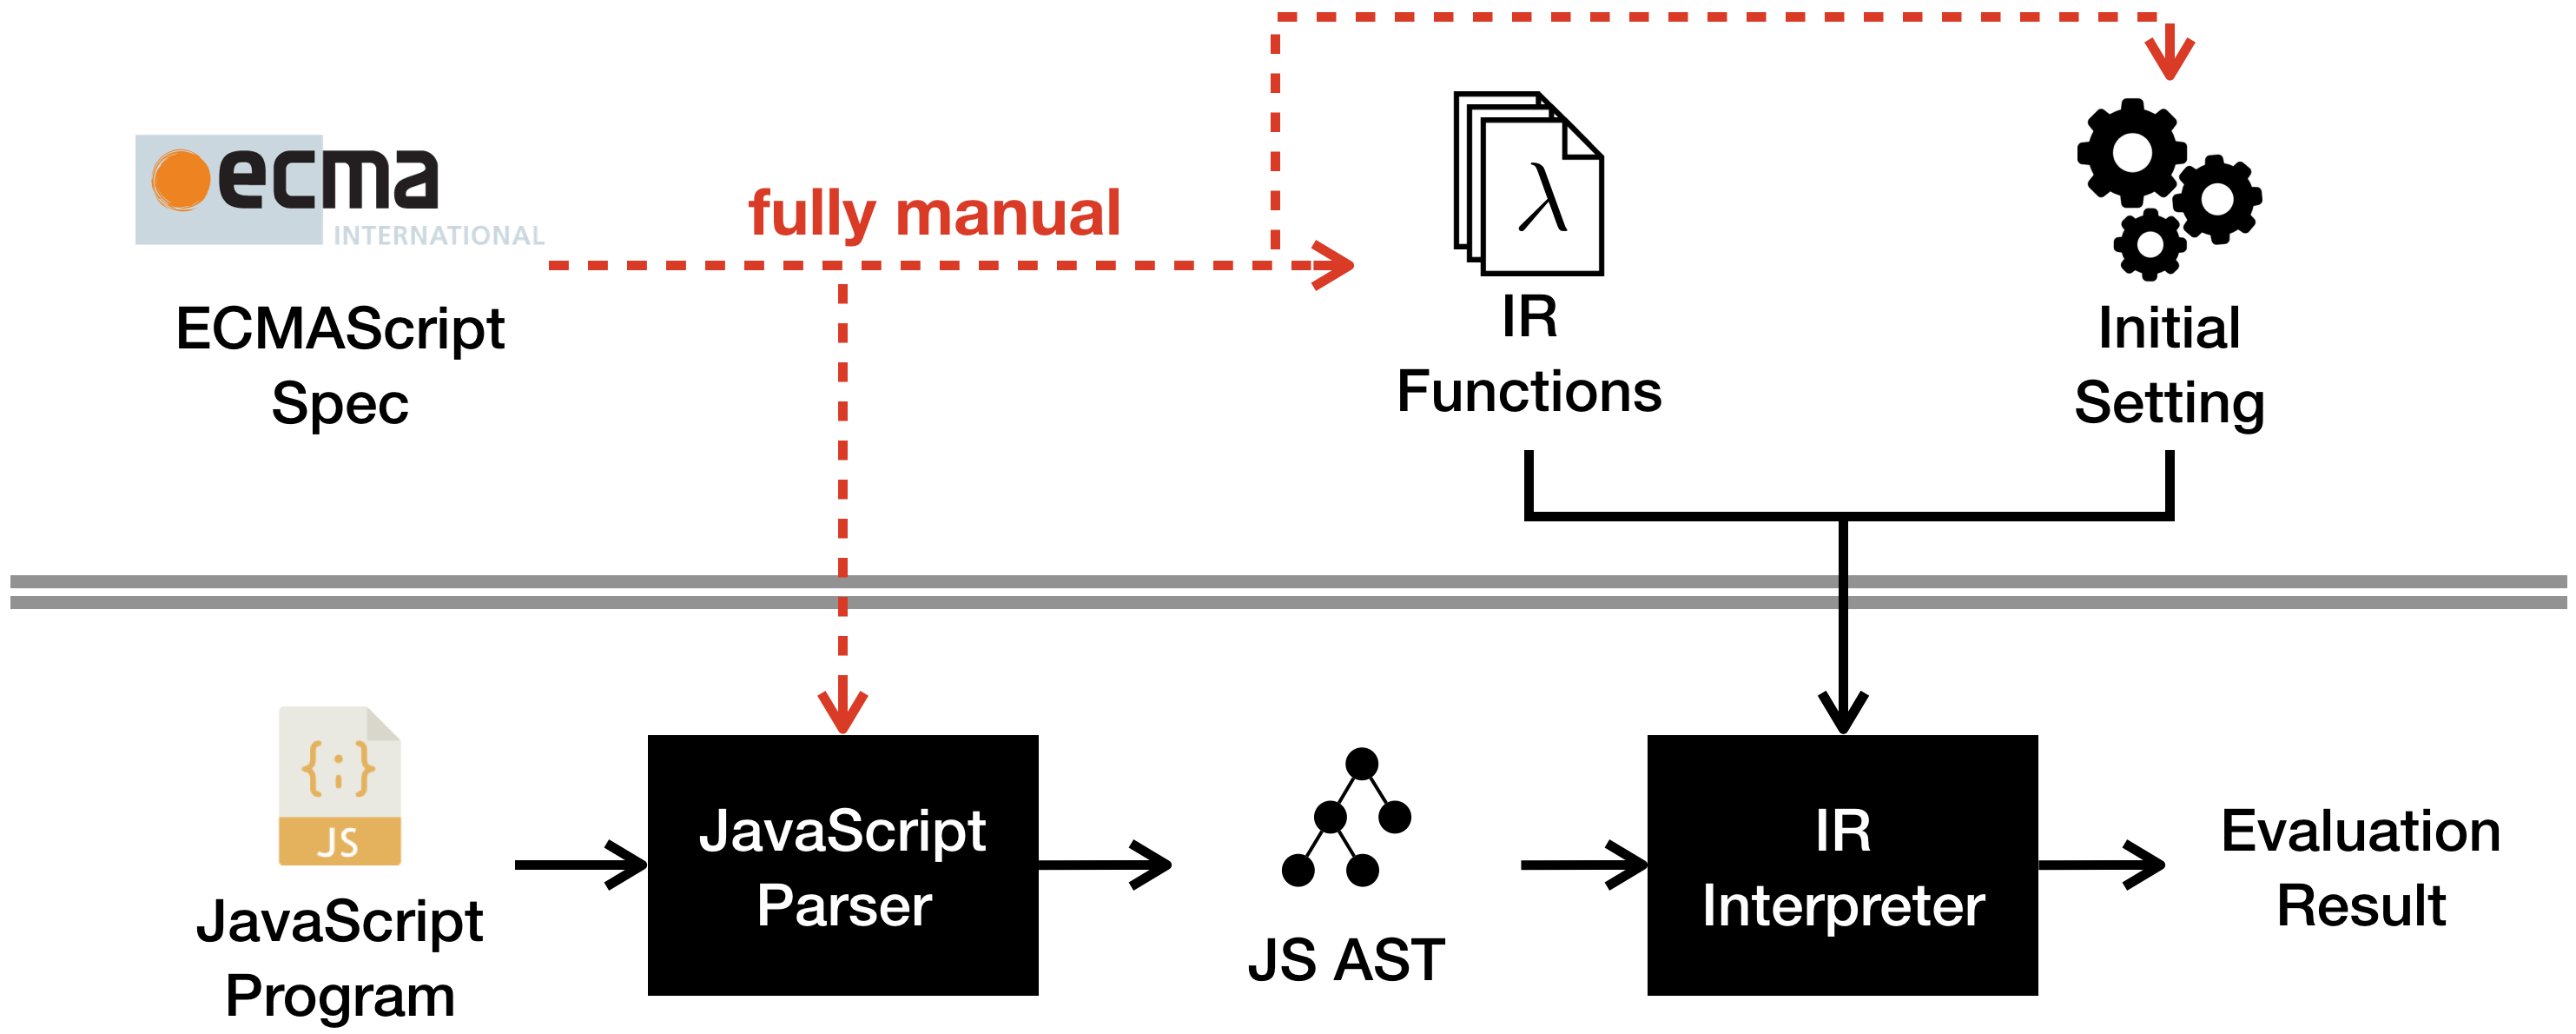
\includegraphics[width=0.5\textwidth]{img/previous.png}
  \caption{Previous approaches of semantics extractions for ECMAScript}
  \label{fig:previous}
\end{figure}

However, the existing JavaScript foraml semantics are fully manually written
by researchers based on ECMAScript specifications. ECMAScript is a standardized language
of JavaScript and its specifications formally define its syntax and semantics.
As described in Figure~\ref{fig:previous}, former researchers implement parser and
describe semantics using their own intermediate representation (IR) according to the ECMAScript
specifications. However, their approaches are fully manual thus excessively labor-intensive
to handle full semantics.

Moreover, it is not suitable approach to cope with the updates of ECMAScript specifications.
Most of full formal semantics of ECMAScript only supports ECMAScript 5.1 that was
released in December 2009. Until 2014 years, it was not big deal because ECMAScript
specifications are rarely updated. However, in late 2014, The Ecma Technical
Committee 39 (TC39) decided to release ECMAScript on a yearly cadence. From the
ECMAScript 6, officially ECMAScript 2015, they updated specifications every years
in June. Now, no researches correctly deal with recent ECMAScript features;
lexical bindings (\( \code{let} \)), spread operator (\( \code{...} \),
classes, for-of operators, async functions, or generators.

To alleviate such problems, we propose \textit{Automatic Semantics Extractor (ASE)}
for ECMAScript specifications. The tool automatically generates JavaScript parser
from syntax provided by ECMAScript specifications. It also extracts formal
JavaScript semantics in semi-automatic ways. It is semi-automatic because
it depends on manually defined \textit{conversion rules}. Each rule describes how abstract
algorithms in specifications are converted into functions of our core language \( \ires \).
However, to save the labor of defininig such rules, we also propose \textit{rule generation assistant}
that suggests new conversion rules based on not yet convertable algorithms.
The assistant help us deal with changed or newly introduced algorithms defined in new version of
ECMAScript specifications as well.

Our main contribution is our tool ASE that mechanizes extraction of JavaScript syntax and semantics
from ECMAScript specifications:
\begin{itemize}
  \item ASE enables to extract the syntax and semantics of ECMAScript 2019,
    which is the latest released version of ECMAScript in June 2019.
    Moreover, we successfully applied our tool into the next proposed version,
    ECMAScript 2020. The official conformance test suite, test262, provides
    \inred{XXXXX} tests for ECMAScript 2020 and we passed \inred{XXXXX} tests
    among them.
  \item ASE is also applicable in-process proposed langauge features in a modular way.
    ECMAScript specifications are open-source based documentations. Thus, anyone
    could propose some new language feautres. Then, the committee carefully inspects
    such proposals and adds them into specifications. Each in-process proposed language
    feature has its own specification and tests. Thus, we apply ASE into the specification
    and evalute the corresponding tests. Among \inred{XX} proposals, we successfully
    pass all the tests in \inred{XX} proposals and partially pass the tests in \inred{XX}
    proposals.
  \item Moreover, all extraction mechanisms in ASE is automatic thus we could use this tool
    to find possible specification errors. We found \inred{X} possible specification errors
    in ECMAScript 2019 and reported them into TC39, which is the Ecma Technical Committee.
    We confirm that all of them are real specification errors.
\end{itemize}
